\documentclass[a4paper, 12pt]{report}
\usepackage[utf8]{inputenc}
\usepackage[T1]{fontenc}

\usepackage{xcolor}
\usepackage{afterpage}

\usepackage{relsize}
\usepackage{moresize}

\usepackage{graphicx}
\usepackage{geometry}

\usepackage{hyperref}
\usepackage{apacite}

% [CHANGE] The title of your thesis. If your thesis has a subtitle, then this
% should appear right below the main title, in a smaller font.
\newcommand{\theTitle}{The first sentence \\
\vspace{0.5em}
the second sentence}
\newcommand{\theSubTitle}{a smaller subtitle}


% [CHANGE] Your full name. In case of multiple names, you can include their
% initials as well, e.g. "Robin G.J. van Achteren".
\newcommand{\theAuthor}{Dewi E. Timman}

% [CHANGE] Your student ID, as this has been assigned to you by the UvA
% administration.
\newcommand{\theStudentID}{12419273}

% [CHANGE] The name of your supervisor(s). Include the titles of your supervisor(s),
% as well as the initials for *all* of his/her first names.
\newcommand{\theSupervisor}{Dr. V. Niculae} % Dr. Ing. L. Dorst

% [CHANGE] The address of the institute at which your supervisor is working.
% Be sure to include (1) institute (is appropriate), (2) faculty (if
% appropriate), (3) organisation name, (4) organisation address (2 lines).
\newcommand{\theInstitute}{
Informatics Institute \\ %Institute for Logic, Language and Computation
Faculty of Science\\
University of Amsterdam\\
Science Park 900 \\ 
1098 XH Amsterdam 
}

% [CHANGE] The semester in which you started your thesis.
\newcommand{\theDate}{Semester 1, 2023-2024}

\begin{document}
\pagestyle{empty}
\begin{center}

\vspace{2.5cm}


\begin{Huge}
% see definition at beginning of document
\theTitle
\end{Huge} \\

\vspace{0.5 cm}

\begin{Large}
\theSubTitle
\end{Large}

\vspace{1.5cm}

% see definition at beginning of document
\theAuthor\\
% see definition at beginning of document
\theStudentID

\vspace{1.5cm}

% [DO NOT CHANGE]
Bachelor thesis\\
Credits: 18 EC

\vspace{0.5cm}

% [DO NOT CHANGE] The name of the educational programme.
Bachelor \textit{Kunstmatige Intelligentie} \\
\vspace{0.25cm}

\includegraphics[width=0.075\paperwidth]{figs/uva_logo} \\
\vspace{0.1cm}

% [DO NOT CHANGE] The address of the educational programme.
University of Amsterdam\\
Faculty of Science\\
Science Park 900\\
1098 XH Amsterdam

\vspace{2cm}

\emph{Supervisor}\\

% see definition at beginning of document
\theSupervisor

\vspace{0.25cm}

% see definition at beginning of document
\theInstitute

\vspace{1.0cm}

% see definition at beginning of document
\theDate

\end{center}
\newpage

\pagenumbering{arabic}
\setcounter{page}{1}
\pagestyle{plain} 

\chapter*{Abstract}
% TODO
\textbf{Key words:} 

\tableofcontents

\chapter{Introduction}
% What am I researching? bruggetje met taal
% \begin{itemize}
%     \item key words $\rightarrow$ sentence
%     \item efficient, accurate, interpretable
%     \item this research: segmentation model more effective, natural, flexible than a bit mask?
% \end{itemize}

What if machines can read our mind? 
If we can give a machine a few key words and let the machine generate a sentence from these key words, our lives would become more productive and efficient. 
This is what autocomplete systems are trying to achieve. 
\textcolor{orange}{The way in which we choose the key words is also important. 
Taking just the first or the last few words of a sentence as key words usually does not capture the full meaning of the sentence.} 
For example, if someone want to capture the meaning of 'I live in Amsterdam' in a few key words, the words 'live Amsterdam' would probably be choosen. 
Thus, the key words come from multiple places in the sentence. 
Therefore, autocomplete systems need to use more complex models to be more efficient and accurate. 

\section{Literature review}
% TODO/delete

\subsection{Autocomplete communication game}

\begin{figure}
    \centering
    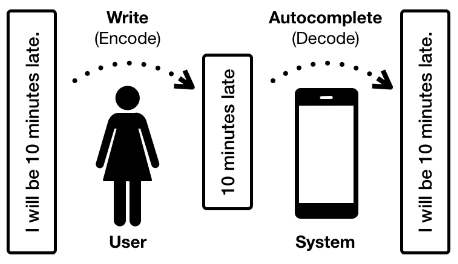
\includegraphics[width=.5\linewidth]{figs/autocomplete_game.png}
    \caption{schematic overview of the communicatoin game. Figure from \protect\citeA{autocomplete}.}
    \label{fig:autocomplete}
\end{figure}

The same autocomplete communication game is considered as in \citeA{autocomplete}. In this game, a human (called user) encodes a sentence into key words. 
These key words are then decoded by a machine (called system) to retrieve the full, initial sentence. 
A schematic overview is given in figure \ref{fig:autocomplete}. 
The communication game is succesfull if the retrieved sentence is the same as the initial sentence. 

More formally, a target sentence $x=(x_1, \dots, x_m)$ is communicated by a user through the key words $z=(z_1, \dots, z_n)$. 
The system then tries to retrieve the target sentence by decoding the key words. 
The target sentence is described by the key words using encoding strategy $q_{\alpha}(z | x)$ and the system decodes the key words by using decoding strategy $p_{\beta}(x|z)$. 

\subsection{Segmentation model}
Why does a segmentation model work?

\subsection{Structured latent variables}
How does the model work? 

\section{Current research}
% Gap
% Research question: To what extend can a segmentation model help by selecting keywords for an auto-complete communication game?

Previous research did not take structure into account \cite{autocomplete, Bar-YossefZiv2011Cqa, SvyatkovskiyAlexey2019PACC}.
Since language is structured, it makes sense to use a structured model as an autocomplete model. 
In this research, we look at how we can use a latent segmentation model to retrieve key words from a sentence. 

\chapter{Method}

\chapter{Results}

\chapter{Conclusion}

\chapter{Discussion}

\bibliography{articles.bib}
\bibliographystyle{apacite}

\end{document}